A photon is a quantized oscillation of an electromagnetic field.  When this
field is in proximity to an interface such as the surface of a metal,
oscillations of free charge can be induced.  If the field is evanescent in
both directions orthogonal to the surface, the oscillations become
localized and are known as surface plasmons (SPs).  Furthermore, if
conditions exist such that the in-plane momentum and phase of the incident
photon and the surface plasmon match, the coupling produces a hybrid
excitation known as surface plasmon polariton (SPP).  An SPP is trapped on
this interface and propagates until it decays; either re-radiating as a
photon or being absorbed into the metal as heat.


\subsection{Wave Equation}
Most of the relevant behavior of SPP propagation can be derived from the
electromagnetic wave equation derived from Maxwell's equations.
\begin{align}
\left(\nabla^2-\mu\epsilon\frac{\partial^2}{\partial t^2}\right)\mathbf{E}&=0
\label{eqn:ewe}
\end{align}
This is the electromagnetic wave equation in terms of the electric field.
Choosing to solve this equation by separation of variables the following
plane wave solutions can be obtained
\begin{align}
 \mathbf{E} ( \mathbf{r}, t ) &= \mathbf{E}_0\, \me^{\mi (\mathbf{k} \cdot \mathbf{r} - \omega t )}
\label{eqn:planewaves}
\end{align}
where $k=\omega/c=\omega\sqrt{\epsilon\mu}$.  In this notation,
$\mathbf{k}$ is the material specific vectorial wavenumber, $\mathbf{r}$ is the
spatial position, $\omega$ is angular frequency, and $t$ is
the dimension of time.
The initial value is chosen with the vectorial constant $\mathbf{E}_0$.
The magnetic field follows the same form
\begin{align}
 \mathbf{H} ( \mathbf{r}, t ) &= \mathbf{H}_0\, \me^{\mi (\mathbf{k}
 \cdot \mathbf{r} - \omega t )}
\end{align} 
but it is orthogonal $\mathbf{E}$ by
\begin{align}
\mathbf{E} \times \mathbf{H} = 0
\end{align}
and the two are mutually orthogonal with the direction of propagation
$\mathbf{k}$.

\subsection{Dispersion Relation}
With plane wave solutions in hand, boundary conditions consistent with a
dielectric-metal interface can be imposed.
At a planar interface, it is convenient to restrict the problem to two
dimensions; in this case the $x$-$z$ plane as shown schematically in
\Figure{fig:kretschmanngeosimplified}.  Since $\mathbf{k}=(k_x,0,k_z)$,
$\mathbf{r}\cdot\mathbf{k}=k_x x + k_z z$ and $\mathbf{E}_0 = (E_x, 0,
E_z)$, the electric field can be written 
\begin{align}
\mathbf{E} ( \mathbf{r}, t ) &= \mathbf{E}_0\, \me^{\mi (\mathbf{k}
\cdot \mathbf{r} - \omega t )}\\
\mathbf{E}(x,z,t)&=\begin{pmatrix}
E_x\\ 0\\ E_z
\end{pmatrix}
\, \me^{\mi(k_{x,i}x+k_{z,i}z-\omega t)}
\label{eqn:planewavexz}
\end{align}
The magnetic field propagates in the same direction with the
same $\mathbf{k}$-vector components, but the direction
$\mathbf{H}$ must be orthogonal to $\mathbf{E}$ by
\Equation{eqn:faradayslaw}
\begin{align}
\mathbf{H} ( \mathbf{r}, t ) &= \mathbf{H}_0\, \me^{\mi (\mathbf{k}
\cdot \mathbf{r} - \omega t )}\\
\mathbf{H}(x,z,t)&=\begin{pmatrix}
0\\ H_y\\ 0
\end{pmatrix}
\, \me^{\mi(k_{x,i}x+k_{z,i}z-\omega t)}
\end{align}
At the interface there are two values for the (complex) permittivity,
$\epsilon_1$ in the dielectric and $\epsilon_2$ in the metal.  Consequently
there are two sets of plane wave solutions
\begin{align}
\left.\begin{aligned}
\mathbf{H}_1(x,z,t) &=
\begin{pmatrix}
0\\
H_{y,1}\\
0
\end{pmatrix} \me^{\mi(k_{x,1}x+k_{z,1}z-\omega t)}\\
\mathbf{E}_1(x,z,t) &=
\begin{pmatrix}
E_{x,1}\\
0\\
E_{z,1}\\
\end{pmatrix} \me^{\mi(k_{x,1}x+k_{z,1}z-\omega t)}
\end{aligned}
\right\}& \quad \text{dielectric}, \epsilon_1\label{eqn:planewavedielectric}\\
\left.\begin{aligned}
\mathbf{H}_2(x,z,t) &=
\begin{pmatrix}
0\\
H_{y,2}\\
0
\end{pmatrix}
\me^{\mi(k_{x,2}x+k_{z,2}z-\omega t)}\\
\mathbf{E}_2(x,z,t) &=
\begin{pmatrix}
E_{x,2}\\
0\\
E_{z,2}\\
\end{pmatrix}
\me^{\mi(k_{x,2}x+k_{z,2}z-\omega t)}
\end{aligned} 
\right\}&\quad \text{metal}, \epsilon_2
\label{eqn:planewavemetal}
\end{align}
where the subscript designates which material the wave equation refers to.
(e.g. $\mathbf{E}_1$ is the electric field in the dielectric, $\mathbf{H}_2$
the magnetic field in the metal, etc.)
Continuity of \Equation{eqn:planewavedielectric} and
\ref{eqn:planewavemetal} at this interface requires that
\begin{align}
E_{x,2}&=E_{x,1}\\
H_{y,2}&=H_{y,1}\\
\epsilon_2 E_{z,2}&=\epsilon_1 E_{z,1}
\end{align}
Applying Ampere's law (\Equation{eqn:ampereslaw}) to the field on the
each boundary gives
\begin{align}
\nabla \times \mathbf{H}_i &= \epsilon_i \frac{\partial \mathbf{E}_i}{\partial t}\\
\begin{pmatrix}
\frac{\partial H_{z,i}}{\partial y} - \frac{\partial H_{y,i}}{\partial z}\\
\frac{\partial H_{x,i}}{\partial y} - \frac{\partial H_{z,i}}{\partial z}\\
\frac{\partial H_{y,i}}{\partial y} - \frac{\partial H_{x,i}}{\partial z}
\end{pmatrix}
&= \begin{pmatrix}
-\mi k_{z,i} H_{y,i}\\
0\\
\mi k_{x,i} H_{y,i}
\end{pmatrix}
\\
&= \begin{pmatrix}
-\mi \omega \epsilon_i E_{x,i}\\
0\\
-\mi \omega \epsilon_i E_{z,i}
\end{pmatrix}
\label{eqn:vectordisp}
\end{align}
where $\mathbf{E}_i$, $\mathbf{H}_i$, $i=1,2$ represent the field in either the
dielectric or the metal.  The vector components of
\Equation{eqn:vectordisp} are therefore related 
\begin{align}
-\mi k_{z,i} H_{y,i} &= -\mi \omega \epsilon_i E_{x,i}\\
k_{z,1} H_{y,1} &= \omega \epsilon_1 E_{x,1}\\
k_{z,2} H_{y,2} &= \omega \epsilon_2 E_{x,2}
\label{eqn:spderivsteptwo}
\end{align}
Since the components of both $\mathbf{E}_i$ and $\mathbf{H}_i$ are
parallel to the interface, $E_{x,i}$ and $H_{y,i}$ are also
continuous. By substitution of $E_{x,i}$, \Equation{eqn:spderivsteptwo} becomes
\begin{align}
\frac{k_{z,1}}{\epsilon_1}H_{y,1}&=\frac{k_{z,2}}{\epsilon_2}H_{y,2}\\ 
\Aboxed{
\frac{k_{z,1}}{\epsilon_1}&=\frac{k_{z,2}}{\epsilon_2} 
}
\label{eqn:sprcondition}
\end{align}
This is the surface plasmon resonance condition.  In terms of
its vector components, the following holds in general for all electromagnetic
waves
\begin{align}
\mathbf{k}^2=\epsilon_i \left(\frac{\omega}{c}\right)^2=k_x^2 + k_{z,i}^2\\
\epsilon_i k_0^2=k_x^2 + k_{z,i}^2
\label{eqn:dispersion1}
\end{align}
Substitution of \Equation{eqn:sprcondition} with the relation 
$k_{x,1}=k_{x,2}$ into \Equation{eqn:dispersion1} allows 
$k_x$ and $k_{z,i}$ to be rewritten in the form of a dispersion relation
\begin{align}
k_x &= k_0\sqrt{\frac{\epsilon_1 \epsilon_2}{\epsilon_1+\epsilon_2}} 
= \frac{\omega}{c}\sqrt{\frac{\epsilon_1 \epsilon_2}{\epsilon_1+\epsilon_2}}\\
k_{z,i} &= k_0\frac{\epsilon_i}{\sqrt{\epsilon_1+\epsilon_2}}
= \frac{\omega}{c}\frac{\epsilon_i}{\sqrt{\epsilon_1+\epsilon_2}}
\end{align}

This relation, shown in \Figure{fig:dispersionrelation}, is useful because
it shows graphically the condition under which SPPs may exist: at the
intersection between the photon light line and corresponding SPP light line
for the medium in question.  Note that for a photon and a plasmon in both a
vacuum and a dielectric, this never happens; the photon assumes $\omega = c
k /\sqrt{\epsilon_i}$ for $i=1,2$, diverging to infinity while the SPP
asymptotically approaches $\omega_p/\sqrt{1+\epsilon_i}$ as $k_x\to\infty$.
However, if light is incident from a dielectric $\epsilon_1$ at an angle
$\theta$, the slope of $\omega(k_x)$ is modified to $c k \sin
\theta/\sqrt{\epsilon_1}$ and the dispersion relations can be matched.
This is the principle exploited by Kretschmann \cite{kretschmann1968} to
excite SPPs with prisms.

There are several regions of interest in \Figure{fig:dispersionrelation},
depending on the relative value of $\epsilon_1$ and $\epsilon_2$.  We first
assume that $\epsilon_1$ is a dielectric with $\epsilon_1\in\mathbb{R}$ and
$\epsilon_1 > 0$ (true for most if not all glass).  In this case, for
$\Re(\epsilon_2)>0$, both $k_x$ and $k_z$ are real.  These are known as
``radiative modes'' -- an SPP mode is supported normal to the interface but
it is not bound there.  For $-\epsilon_1<\Re(\epsilon_2)<0$, $k_z$ is real
and $k_x$ imaginary.  The SPP is not confined to the interface and decays
evanescently there; this is known as a ``quasi-bound mode''  However, for
$\Re(\epsilon_2)<-\epsilon_1$, $k_x$ is real and $k_z$ is imaginary.  This
indicates the SPP is localized at the interface in $z$ while having a
propagating solution in $x$, and is exactly the condition we wish to match.
\begin{figure}[ht]
\centering
\begin{tikzpicture}
\begin{axis}[
xlabel=$k_x$,
ylabel=$\omega$,
xmin=0,
xmax=0.6e8,
ymin=0.75e15,
ymax=6.5e15,
thick,
width=0.75\textwidth,
height=0.75\textwidth,
minor tick num=2,
legend pos = south east,
legend style = { cells = {anchor=west} },
clip=false,
]
\addplot[] file {figures/data/kx_photon_glass.dat}
node [anchor=south west,yshift=-10pt]{$ck/\sqrt{\epsilon_1}$}; 
%\textattachfile{figures/data/kx_photon_glass.dat}{}
\addlegendentry{photon/dielectric}

\addplot[] file {figures/data/kx_photon_glass_tilted.dat}
node [anchor=south west,yshift=-10pt]{$ck \sin \theta /\sqrt{\epsilon_1}$};
\addlegendentry{photon/dielectric angle}

\addplot[] file {figures/data/kx_photon_vacuum.dat}
node [anchor=south west,yshift=-10pt]{$ck$}; 
\addlegendentry{photon/vacuum}

\addplot[] file {figures/data/kx_sp_metal_glass_lower.dat};
\addlegendentry{SPP/dielectric}

\addplot[] file {figures/data/kx_sp_metal_vacuum_lower.dat};
\addlegendentry{SPP/vacuum}

\addplot[] file {figures/data/kx_sp_metal_glass_upper.dat};
\addplot[] file {figures/data/kx_sp_metal_vacuum_upper.dat};

\addplot[,dashed] coordinates { (6e7,5.819396016587478e+15) (0,5.819396016587478e+15) }
node [anchor=east,xshift=-15pt]{$\omega_p$}; 

\addplot[,dashed] coordinates { (6e7,5.461458222933e+15) (0,5.461458222933e+15) }
node [anchor=east,xshift=-15pt]{$\omega_p/\sqrt{2}$}; 

\addplot[,dashed] coordinates { (6e7,4959276840790959) (0,4959276840790959) }
node [anchor=east,xshift=-15pt]{$\omega_p/\sqrt{1+\epsilon_2}$}; 


\draw [decorate,decoration={brace,amplitude=8pt}] (axis cs:6e7,6.5e+15)--(axis cs:6e7,5.819396016587478e+15)
node [midway,anchor=west,xshift=10pt,align=left]{radiative modes\\ $k_x,k_z \in \mathbb{R}$};

\draw [decorate,decoration={brace,amplitude=8pt}] (axis cs:6e7,5.819396016587478e+15)--(axis cs:6e7,4959276840790959)
node [midway,anchor=west,xshift=10pt,align=left]{quasi-bound modes\\ $k_x \in \mathbb{I}$,  $k_z \in \mathbb{R}$};

\draw [decorate,decoration={brace,amplitude=8pt}] (axis cs:6e7,4959276840790959)--(axis cs:6e7,0.75e+15)
node [midway,anchor=west,xshift=10pt,align=left]{bound modes\\ $k_x \in \mathbb{R}$\\ $k_z \in \mathbb{I}$};

\end{axis}
\end{tikzpicture}
\caption{Dispersion relation for photons and plasmons.  Conditions under
which SPPs may occur at the intersection between the photon light line and
corresponding SPP light line for the medium in question.  Based on a
similar plot found in \cite{shsongspp}.}
\label{fig:dispersionrelation}
\end{figure}
Fix the colors here.
The dispersion diagram relates the time-variation of the wave (given by its
frequency omega) to the spatial variation of the wave (given by its
wave-vector kx)

\subsection{Resonance Condition}
The resonance condition requires the dispersion relation for an
incident photon intersect the dispersion relation for SPPs, matching both
their in-plane momentum and phase.  This can be achieved by if the photon
is indecent through a dielectric at an $\theta_\text{sp}$, causing its phase
velocity $\omega/k_x$ to be reduced to  $\omega/k_x = c/(\sqrt{\epsilon_1}
\sin \theta)$.  One simple and popular prism coupled configuration (the one
which will be employed throughout this work) which is able to match these
conditions is known as the Kretschmann attenuated total reflection (ATR)
configuration, and is shown schematically in \Figure{fig:kretschmanngeo}.
Here a thin ($\sim \SI{50}{\nano\meter}$) metal film is deposited on to the
hypotenuse of a dielectric prism, and the totally internally reflected
light evanescently excites SPPs.  The SPP resonance condition for this
system is
\begin{align}
k_\text{sp}=k_0 \sqrt{\epsilon_1} \sin \theta_\text{sp} 
\end{align}
Note that practically this can only occur when both the width of the metal
layer $d$ is less than the evanescent decay in that direction
$\Im(1/k_{z,2})$ (causing the metal to be nearly transparent) and the
incident light satisfies the condition for total internal reflection.  This 
is approximately when
\begin{align}
\theta>\arcsin\left(\sqrt{\frac{\epsilon_1}{\epsilon_3}}\right)
\end{align} 
In practice the resonance angle $\theta_\text{sp}$ is most easily found by
numerically evaluating the Fresnel relations discussed in the following
section.

\subsection{Fresnel Relations}
Many features of surface plasmon resonance can be predicted using the
Fresnel relations and the transfer matrix method (TMM) for multilayer
stacks.
The Fresnel reflection coefficient $\tilde{r}$ is defined as the ratio of the
reflected beam $\tilde{E}_r$ to the incident beam
$\tilde{E}_i$
\begin{align}
\tilde{r} &= \frac{\tilde{E}_r}{\tilde{E}_i}
\end{align}
Here the presence of a tilde $\sim$ indicates a function in the (spatial)
frequency domain.  For multilayer systems, this is found through
the transfer matrix method where the $i$th matrix $M_i$ is
\begin{align}
M_i = \left(\begin{array}{cc}
\cos \sigma_i & \mi \sin \sigma_i / \gamma_i\\
\mi \gamma_i \sin \sigma_i & \cos \sigma_i
\end{array}\right)
\label{eqn:tmm}
\end{align}
and the system matrix $M_s = M_1 M_2 \ldots M_{n-1} M_n$.  In the above
representation
\begin{align}
\left.\begin{aligned}
\gamma_i &= \sqrt{\epsilon_i} k_{z,i}\\
\sigma_i &= k_{z,i} \sqrt{\epsilon_i} d_i
\end{aligned}
\right\}& \quad \text{for TE Polarization}\\
\left.\begin{aligned}
\gamma_i &= \sqrt{\epsilon_i}/k_{z,i}\\
\sigma_i &= k_{z,i} \sqrt{\epsilon_i} d_i
\end{aligned}
\right\}& \quad \text{for TM Polarization}
\end{align}
The elements of the resulting elements of $M_s$, $M_{i,j}$ are then
substituted into the formula
\begin{align}
\tilde{r}=
\frac{\gamma_1 M_{11}+\gamma_1 \gamma_3 M_{12} - M_{21} - \gamma_3 M_{22}}
{\gamma_1 M_{11}+\gamma_1 \gamma_3 M_{12} + M_{21} + \gamma_3 M_{22}}
\end{align}
With a bit of algebra, the Fresnel reflection for an arbitrary number of
layers in the case of TM polarization can be found to be
\begin{align}
\tilde{r}_{j,l,m \ldots n} = 
\frac{\tilde{r}_{j,l} + \tilde{r}_{l,m \ldots n} \me^{2 \mi k_{z,l} d_l}}
{1+\tilde{r}_{j,l} \tilde{r}_{l,m \ldots n} \me^{2 \mi k_{z,l} d_l}}
\label{eqn:bertnlayer}
\end{align}
where $d_l$ is the thickness of the $l$th metal layer and 
\begin{align}
\tilde{r}_{i,j}&=
\left.\left(\frac{k_{z,i}}{\epsilon_i}-\frac{k_{z,j}}{\epsilon_j}\right)
\middle/
\left(\frac{k_{z,i}}{\epsilon_i}+\frac{k_{z,j}}{\epsilon_j}\right)\right.\\
&=\frac{\epsilon_j k_{z,i}-\epsilon_i k_{z,j}}
{\epsilon_j k_{z,i}+\epsilon_i k_{z,j}}
\end{align}
is the two layer Fresnel relation.  \Equation{eqn:bertnlayer} may be
recursively applied for any number of layers.  There are computational
limits to this approach which make it unsuitable for large multilayer
stacks; in such a case methods based on \Equation{eqn:tmm} are more
appropriate.  For convience we state the three layer Fresnel reflectivity
$\tilde{r}_{123}$, based on the geometry of \Figure{fig:kretschmanngeo}
\begin{align}
\tilde{r}_{123}(k_x) &=
\frac{
  (\epsilon_2 k_{z,1}+\epsilon_1 k_{z,2})(\epsilon_3 k_{z,2}-\epsilon_2 k_{z,3})
+ (\epsilon_2 k_{z,1}-\epsilon_1 k_{z,2})(\epsilon_3 k_{z,2}+\epsilon_2 k_{z,3})\,
\me^{\mi 2 k_{z,2} d_2}
}
{
  (\epsilon_2 k_{z,1}+\epsilon_1 k_{z,2})(\epsilon_3 k_{z,2}+\epsilon_2 k_{z,3})
+ (\epsilon_2 k_{z,1}-\epsilon_1 k_{z,2})(\epsilon_3 k_{z,2}-\epsilon_2 k_{z,3})\,
\me^{\mi 2 k_{z,2} d_2}
}\\
&=
\frac{\tilde{r}_{12}+\tilde{r}_{23}\, \me^{\mi 2 k_{z,2} d_2}} {1+\tilde{r}_{12} \tilde{r}_{23} \me^{\mi 2 k_{z,2} d_2}}
\label{eqn:fresnel123}
\end{align}
Note that factor of two in the exponential: the SPP accumulates phase
through the metal film twice (once upon excitation, another upon decay).
In this equation, $k_{z,i}$ can be equivalently expressed either as a
function of incident angle $\theta$ or $k_x$
\begin{align}
k_{z,i} &= k_0 \sqrt{\epsilon_i - \epsilon_1 \sin \theta}\\
&= \sqrt{k_0^2\epsilon_i - k_x^2}
\end{align}

\begin{figure}
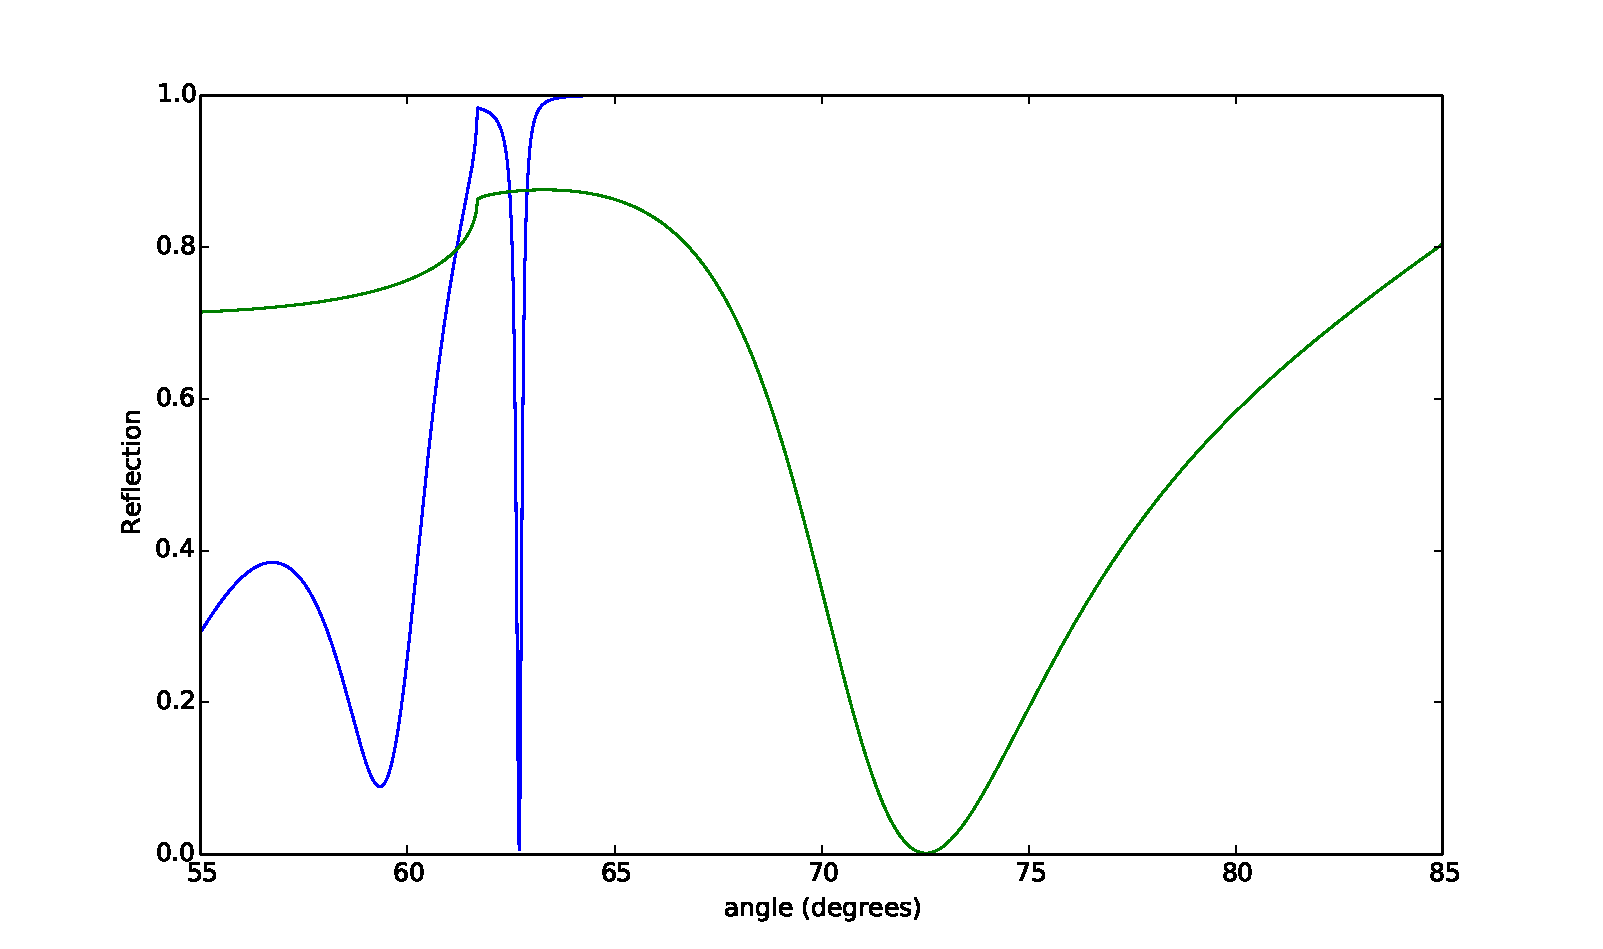
\includegraphics[width=0.9\textwidth,keepaspectratio]{figures/fresnelspp_ersatz.pdf}
\caption{spp and lrspp, gold on cytop}
% bk7 hemisphere 
%x0 = array([ 1250e-9, 16e-9 ])
%out = array([ fresnel(t,x0) for t in theta ])
%x0 = array([ 1150e-9, 45e-9 ])
% data in figures/data/spp_fresnel.dat
\end{figure}

\subsection{Physical Properties}
Physical properties of SPP propagation are derived from $k_x$ and $k_z$.
Since the SPP is confined to the plane of the metal, the surface plasmon
wavelength $\lambda_\text{sp}$ is defined in terms of the real part of
$k_x$
\begin{align}
\lambda_\text{sp} &= \frac{\lambda_0}{2 \pi} k_x\\
& = \Re\left(\sqrt{
  \frac {\epsilon_1+\epsilon_2}
   {\epsilon_1 \epsilon_2 \lambda_0^2}
}\right)
\end{align}
when $k_x$ is imaginary, \Equation{eqn:planewavexz} is evanescent in
$x$ and the SPP decays with a characteristic $1/\me$ lifetime
$\Im(1/(2k_x)$.  Similarly, when $k_{z,i}$ is imaginary, the
$1/\me$ evanescent decay into either the metal or vacuum is given by
$\Im(1/k_{z,i})$.  A table of these properties for many different SPP
excitation configurations is found in \Appendix{ref:physicalproperties}.

\section{Long Range Surface Plasmon Polaritons}
The typical propagation distances for SPPs in the three layer Kretschmann
configuration are on the order of $\SI{30}{\nano\meter}$ for Ag films and
$\SI{6}{\nano\meter}$ for Au films.  The reason for this is the electric
field extends into the metal and the real part of the metal's dielectric
function damps the SPP oscillation, causing it to decay as heat.  However,
if we are able to expel the SPP evanescent field from the metal region, the
propagation distances can be extended orders of magnitude.  These are
called \textit{long range surface plasmon polaritons} (LRSPPs), and in
terms of our geometry can be excited in one of two ways.

symmetric vs asymmetric spps

\subsection{Symmetric Configuration}
Cytop coating crap
\subsection{Photonic Crystal Configuration}

\section{Typical Response}
some pictures of spp prop